\documentclass{swjtuthesis}

\addbibresource{example.bib}
\nocite{*}

\begin{document}

\score{85}
\taskpurpose{随着大数据的发展、以及国家推动实施大数据的号召,各个行业都应加强信息化和工业化深度的融合,加快进入数字经济时代。当前网络购物已经成为人们生活不可分割的一部分,但面对琳琅满目的商品,人们需要去浏览和对比各个店铺的信息,如好评,差评,购买人数等繁琐的步骤。通过分析网购活动,收集每个商家的所有有用信息,并对这些大数据进行分析,将对消费者有用的信息直接简单明了的展示给客户。本课题拟以京东购物网站为例,利用Python、Scrapy爬虫框架、Redis数据库以及Django Web框架、Pandas数据分析等技术,开发实现一套以数据挖掘及分析为核心的京东商城数据分析系统。
}
\tasktodo{
    本课题拟采用Python、Scrapy爬虫框架、Redis数据库以及Django Web框架、Pandas数据分析等技术开发。具体任务如下:\hspace*{\fill}
\\
     (1) 研究完成该系统的关键技术:Scarpy+Redis实现分布式爬虫,Pandas实现数据分析,Django实现web展示;\hspace*{\fill}\\
     (2) 对京东商城进行网页源代码分析以及爬取所需信息,对所用信息进行分析提炼,以词云,图表形式展现出来;\hspace*{\fill}\\
     (3) 使用python编程语言,实现数据挖掘、数据分析、前端展示三大部分。
}
\taskachievement{
    本论文支撑本专业以下毕业要求的达成:(1)能够通过查阅和分析文献,为软件系统及工程的问题求解寻找方案,并认识到所求解的问题具有多种可能的解决途径(指标点2.3);(2)能够针对特定需求确定目标,设计软件系统框架、组成模块,合理组织/存储数据,基于适当的模型进行软件系统设计与实现,并体现一定的创新意识(指标点3.2);(3)能够在解决方案中从技术、非技术(如经济、社会、健康、安全、法律、文化以及环境等)角度,对设计方案的可行性进行评价和分析(指标点3.3);(4)能够采用科学方法对软件系统及工程问题进行研究,通过实验对比、文献综合、归纳整理得到合理有效结论,并对其进行规范表述(指标点4.3);(5)能够利用开发环境和工具,对软件系统及工程问题进行模拟仿真和数据分析(指标点5.3);(6)能识别、分析、评价特定需求的软件系统在设计和实现中对社会、健康、安全、法律以及文化的影响,并明确自己应承担的责任(指标点6.2);(7)能够评价软件系统设计、开发、运行和维护对环境保护和社会持续发展的影响(指标点7.2);(8)能够通过口头、文稿、图表等方式、陈述和表达自己的观点,能够就软件系统及工程问题与同行和相关人员进行交流(指标点10.1);(9)能够根据对工作内容和过程的记录与整理,撰写技术报告和设计文稿、陈述发言或回应质询(指标点10.2);(10)了解软件系统工程管理原理与经济决策方法,理解软件系统项目的组织模式和实施过程,掌握项目管理原理和内容(指标点11.1);(11)正确认识自主学习的必要性和重要性,认识到本专业是一个发展迅速的学科,具有自主学习和终身学习的意识(指标点12.1);(12)具备自主学习新技术和新方法的能力,能够通过学习不断提高、适应信息技术和职业的发展(指标点12.2)。 
}

\taskplana{查阅相关资料文献、开题}{4}
\taskplanb{项目需求分析与设计}{3}
\taskplanc{项目编码、测试}{5}
\taskpland{整理相关资料、撰写毕业论文}{3}
\taskplane{修改论文、准备答辩资料}{2}
\taskplanl{根据学校统一安排进行答辩}


\title{毕业设计标题:Thesis' Title}
\grade{2017级}
\stunum{1234567890}
\author{张三}
\major{软件工程}
\class{软件2016-3班}
\instructor{李四}
\department{信息科学与技术学院}
\maketitlepage

\makeais
\makecua
\makeevaluatepage
\makescorepage
\maketaskpage

\startabstract
\keywords{关键词1;关键词2;关键词3}
\enkeywords{kw1; kw2; kw3; kw4; kw5}
\begin{abstract}
    Web信息的爆炸性增长使Internet成为我们获取信息资源的重要途径,而在全球一体化的今天,人们对翻译质量和翻译速度的要求也日趋严格。网络上拥有大量的双语对照信息,而传统的搜索引擎无法对其进行充分的利用。因此,本文从搜索技术和翻译技术上进行研究,提出了一个基于双语翻译的搜索引擎系统。

    本文利用Heritrix和Lucene工具,在计算机辅助翻译的基础上利用搜索引擎技术,实现检索具有双语对照信息的网页。本文主要研究如何从海量信息库中爬取网页资源,设计出识别双语网页和提取双语语料的方法,并构造出合适的索引器和检索器,通过用户接口将网页信息输出给用户。   
\end{abstract}
\begin{enabstract}
    The explosive growth of Web information makes Internet be an important way to obtain information resources for us. Because of today’s global integration, the quality and speed of translation work are becoming stricter and stricter. There is a large amount of bilingual information in the network, but traditional search engines cannot make full use of them. Therefore, this thesis studies search and translation technologies and proposes a search engine system based on bilingual translation.

    This thesis realized searching Web pages that have bilingual information, and combined computer-aided translation technology with search engine technology with Heritrix and Lucene tools. This thesis mainly researches how to crawl Web resources from massive information, and designs a method for recognizing bilingual Web pages and extracting bilingual corpora. The search engine implements in this thesis will output Web information to users through the user interface with the help of indexers and searchers.

    The explosive growth of Web information makes Internet be an important way to obtain information resources for us. Because of today’s global integration, the quality and speed of translation work are becoming stricter and stricter. There is a large amount of bilingual information in the network, but traditional search engines cannot make full use of them. Therefore, this thesis studies search and translation technologies and proposes a search engine system based on bilingual translation.

    This thesis realized searching Web pages that have bilingual information, and combined computer-aided translation technology with search engine technology with Heritrix and Lucene tools. This thesis mainly researches how to crawl Web resources from massive information, and designs a method for recognizing bilingual Web pages and extracting bilingual corpora. The search engine implements in this thesis will output Web information to users through the user interface with the help of indexers and searchers.
\end{enabstract}

\maketot

\startmainmatter

\chapter{绪 论}
\section{背景与意义}

这是正文第一{\heiti 黑体 \textbf{粗体}}段\supercite{rosen2000multiprotocol}。
\textit{斜体}

\begin{figure}[hbt]
    \centering
    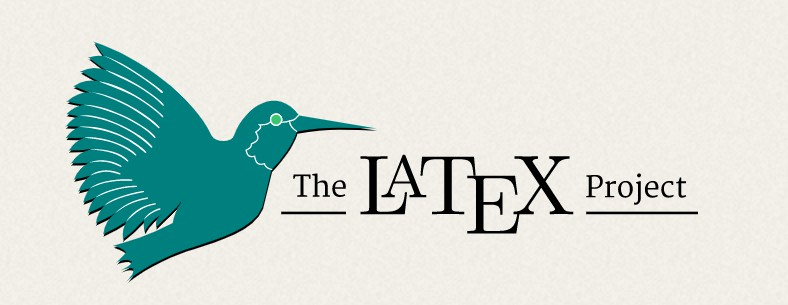
\includegraphics[width=0.7\linewidth]{example.jpg}
    \caption{测试图片}
\end{figure}

\begin{table}[hbt]
    \centering
    \caption{测试表格}
    \begin{tabular}{ c|c|c } 
    \hline
    cell1 & cell2 & cell3 \\
    \hline
    cell4 & cell5 & cell6 \\ 
    \hline
    cell7 & cell8 & cell9 \\ 
    \hline
    \end{tabular}
\end{table}

\begin{equation}
    E=mc^2
\end{equation}

\chapter{标题}
\section{一级节标题}
\subsection{二级节标题}
\subsection{二级节标题}
\subsection{二级节标题}
\section{一级节标题}
\subsection{二级节标题}
\subsection{二级节标题}
\subsection{二级节标题}
\section{本章小结}

\chapter{标题}
\section{一级节标题}
\subsection{二级节标题}
\subsection{二级节标题}
\section{一级节标题}
\subsection{二级节标题}
\subsection{二级节标题}
\section{本章小结}

\makebackmatter

\end{document}